\documentclass[tikz,border=5pt]{standalone}
\usepackage{pgfplots}
\usepackage{amsmath}
\pgfplotsset{compat=1.18}

\definecolor{corba}{HTML}{365FB3}
\definecolor{maxim}{HTML}{B91C1C}
\definecolor{minim}{HTML}{D97706}
\definecolor{extrem}{HTML}{374151}

\begin{document}
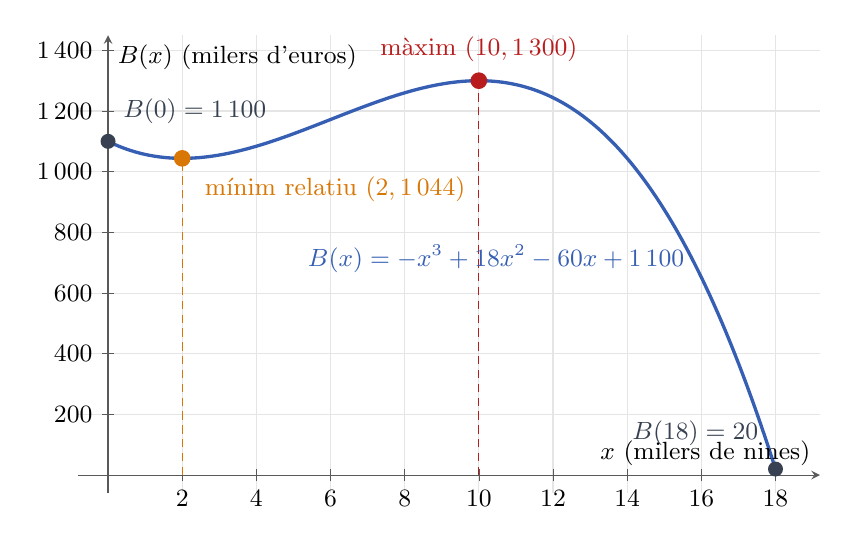
\begin{tikzpicture}
  \begin{axis}[
    width=11cm,
    height=7.4cm,
    axis lines=middle,
    xmin=-0.8,
    xmax=19.2,
    ymin=-60,
    ymax=1450,
    xlabel={$x$ (milers de nines)},
    ylabel={$B(x)$ (milers d'euros)},
    xtick={0,2,4,6,8,10,12,14,16,18},
    ytick={0,200,400,600,800,1000,1200,1400},
    scaled y ticks=false,
    yticklabel style={/pgf/number format/fixed,/pgf/number format/1000 sep={\,}},
    grid=major,
    grid style={black!10},
    axis line style={black!65},
    tick style={black!65},
    tick label style={font=\small},
    label style={font=\small},
    clip=false,
  ]
    \addplot[corba, very thick, domain=0:18, samples=240]
      {-x^3+18*x^2-60*x+1100};

    \draw[minim, densely dashed]
      (axis cs:2,0) -- (axis cs:2,1044);
    \draw[maxim, densely dashed]
      (axis cs:10,0) -- (axis cs:10,1300);

    \addplot[only marks, mark=*, mark size=2.5pt, extrem]
      coordinates {(0,1100) (18,20)};
    \addplot[only marks, mark=*, mark size=2.8pt, minim]
      coordinates {(2,1044)};
    \addplot[only marks, mark=*, mark size=2.8pt, maxim]
      coordinates {(10,1300)};

    \node[anchor=south west, text=extrem, font=\small]
      at (axis cs:0.15,1125) {$B(0)=1\,100$};
    \node[anchor=north west, text=minim, font=\small]
      at (axis cs:2.35,1015) {mínim relatiu $(2,1\,044)$};
    \node[anchor=south, text=maxim, font=\small]
      at (axis cs:10,1330) {màxim $(10,1\,300)$};
    \node[anchor=south east, text=extrem, font=\small]
      at (axis cs:17.8,65) {$B(18)=20$};

    \node[anchor=north east, text=corba, font=\small]
      at (axis cs:15.8,790) {$B(x)=-x^3+18x^2-60x+1\,100$};
  \end{axis}
\end{tikzpicture}
\end{document}
